\documentclass[10pt, final, twoside]{article}

\usepackage[T2A]{fontenc}
\usepackage[utf8x]{inputenc}

\usepackage[russian, english]{babel}

\usepackage{float}
\usepackage[default]{lato}
\usepackage{textcomp}
\usepackage{amsmath, amssymb}
\usepackage{hyperref}
\usepackage[dvipsnames]{xcolor}
\usepackage[document]{ragged2e}
\usepackage[export]{adjustbox}
\usepackage{setspace}
\setstretch{1.5}

\usepackage{vmargin}
\setpapersize{A4}
\setmarginsrb{1cm}{1cm}{1cm}{1cm}{0pt}{0mm}{0pt}{13mm}

\usepackage{graphicx}

\renewcommand\arraystretch{1.8}
\newcommand{\No}{\textnumero}

\definecolor{darkgray2}{HTML}{434343}
\definecolor{darkgray4}{HTML}{cccccc}
\newcommand{\skill}[1]{\colorbox{darkgray4}{\textcolor{darkgray2}{#1}}}

\sloppy
\begin{document}
  \begin{minipage}{0.15\textwidth}\fbox{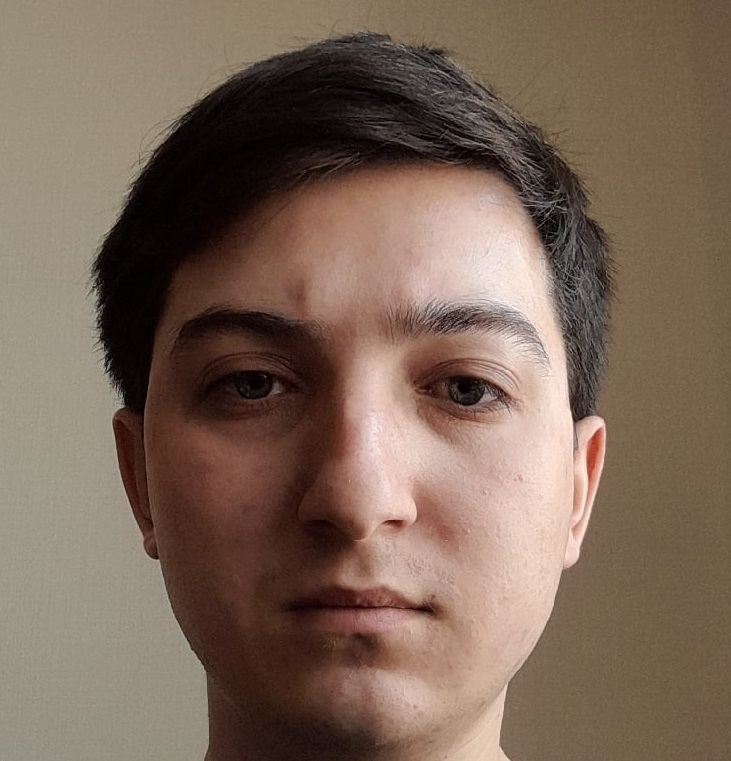
\includegraphics[width=\linewidth, right]{cv_photo.jpg}}\end{minipage}
  \begin{flushright}\section*{\textcolor{darkgray2}{Ханнанов Ленар Ильнурович}}\end{flushright}
  \vspace*{-5.5mm}
  \par\noindent\rule{\textwidth}{0.1pt}
  \textbf{Дата рождения:} 28 октября 2000.
  
  \textbf{Занятость:} проектная работа, стажировка, частичная занятость.
  
  \textbf{График работы:} удаленная работа, гибкий график, сменный график.

  \subsection*{\textcolor{darkgray2}{Контакты}}
  \vspace*{-5.5mm}
  \par\noindent\rule{\textwidth}{0.1pt}
  \begin{itemize}
    \item[\textcolor{MidnightBlue}{\textbullet}] \textcolor{MidnightBlue}{\underline{\url{https://t.me/come_ill_foo}}}
    \item[\textcolor{MidnightBlue}{\textbullet}] \href{mailto:khannanov2000@yandex.ru}{\textcolor{MidnightBlue}{\underline{khannanov2000@yandex.ru}}}
    \item[\textcolor{MidnightBlue}{\textbullet}] \href{tel:79279334902}{+7(927)933-49-02}
  \end{itemize}

  \begin{itemize}
    \item \textbf{195298}, Санкт-Петербург, м. Ладожская
  \end{itemize}

  
  \subsection*{\textcolor{darkgray2}{Опыт работы}}
  \vspace*{-5.5mm}
  \par\noindent\rule{\textwidth}{0.1pt}
  \begin{table}[H]
    \begin{tabular}{ll}
      08.2021--09.2021 & \textbf{RusEFI}\\
                       & \textbf{Программист}\\
                       & 1. Исправлял баги в приложении на Java+Swing\\
                       & 2. Осуществлял миграцию с системы сборки Apache Ant на Gradle 
    \end{tabular}
  \end{table}
  \begin{table}[H]
    \begin{tabular}{ll}
      02.2022--08.2022 & \textbf{ООО "Скайтек"}\\
                       & \textbf{Программист}\\
                       & 1. Проверял работу пропатченного ядра Linux (5.11, 5.17) на эмуляторе   Renode\\
                       & для микроконтроллеров на базе RISC-V архитектуры с MMU (BeagleV) и бе   (Kenryte K210)\\
                       & 2. Настраивал маршрутизатор iRZ R2 на общение по COM-порту    существующим бэкендом\\
                       & на Python (Flask)
    \end{tabular}
  \end{table}
  

  \subsection*{\textcolor{darkgray2}{Образование}}
  \vspace*{-5.5mm}
  \par\noindent\rule{\textwidth}{0.1pt}
  \begin{table}[H]
    \begin{tabular}{ll}
      2019--2023 & \textbf{НИУ ИТМО, Санкт-Петербург, 09.03.04, ПИИКТ, Системное Программное Обеспечение}
    \end{tabular}
  \end{table}

  \subsection*{\textcolor{darkgray2}{Ключевые навыки}}
  \vspace*{-5.5mm}
  \par\noindent\rule{\textwidth}{0.1pt}
    \skill{C/C++} \skill{Linux} \skill{Git} \skill{Python} \skill{PostgreSQL} \skill{Assembler} \skill{Java} \skill{Redis} \skill{Vue 3} \skill{Flask} \skill{Verilog HDL} \skill{Bash} \skill{GNU Make} \skill{Gradle} \skill{Binutils}
    
  \subsection*{\textcolor{darkgray2}{О себе}}
  \vspace*{-5.5mm}
  \par\noindent\rule{\textwidth}{0.1pt}
  
Бакалавриат (4 курс). В свободное время люблю поигрывать в видеоигры.

Ниже расписал, чем увлекаюсь в профессиональной деятельности, включил все, что как-то смотрел, трогал в реальной жизни (это в основном про микроконтроллеры) и изучал в рамках университетской программы.

\par\noindent\rule{\textwidth}{0.1pt}

В основном пишу на языках низкого уровня типо ассемблера архитектур x86\_64 и базово RISC-V; и C. Поэтому увлекаюсь вопросами встроенных системам и IoT. Среди проектов у меня в основном различные учебные проекты и модули устройств для ядра Linux:
\begin{enumerate}
  \item Символьные, блочные, сетевые модули устройств для ядра Linux (работа проверялась в основном на Ubuntu 20.04-22.04) - \url{https://github.com/Come1LLF00/device-drivers-development}
  \item Агломеративная иерархическая кластеризация на C (\url{https://github.com/Come1LLF00/nuke}), так что да я знаком с некоторыми методами машинного обучения
  \item Многопоточное приложение с использованием Posix Threads (\url{https://gitlab.se.ifmo.ru/system-software/ifmo-spring-2022/posix/come_ill_foo})
  \item Аллокатор памяти с использованием системного вызова mmap (\url{https://gitlab.se.ifmo.ru/come_ill_foo/assignment-memory-allocator})
  \item Сепия фильтр с использованием ассемблерных SIMD инструкций на архитектуре x86\_64 (\url{https://gitlab.se.ifmo.ru/come_ill_foo/assignment-sepia-filter})
  \item Базовые функции ввода-вывода на ассемблере x86\_64 (\url{https://gitlab.se.ifmo.ru/come_ill_foo/assignment-1-io-library})
  \item Разворот картинки в формате BMP на C (\url{https://gitlab.se.ifmo.ru/come_ill_foo/assignment-image-rotation})
  \item Компилятор Pascal-подобного языка, строящий AST дерево и транслирующий его в трёхадресный код. Используются flex и bison (\url{https://github.com/Come1LLF00/student-pc})
  \item Знаком с форматами исполняемых файлов PE и ELF
\end{enumerate}

\par\noindent\rule{\textwidth}{0.1pt}

Знаком с отладочной платой Xilinx Nexys 4 DDR и писал для нее прошивки на Verilog HDL в Vivado Design Suite (также знаком с Icarus Verilog):
\begin{enumerate}
  \item Доработка однотактового RISC-V процессора своими инструкциями (\url{https://github.com/Come1LLF00/schoolRISCV})
  \item Модуль вычисляющий математическую функцию (использует семисегментный индикатор и переключатель для взаимодействия с пользователем) - \url{https://github.com/Come1LLF00/rtl_math_acc}
\end{enumerate}

\par\noindent\rule{\textwidth}{0.1pt}

Также писал CRUD с использованием Java + Spring Boot + Vue.js + PostgreSQL + REST API:
\begin{enumerate}
  \item Фронтенд (\url{https://github.com/Come1LLF00/looking-glass})
  \item Бэкенд (\url{https://github.com/Come1LLF00/alicization})
  \item Скрипты для создания модели в БД (\url{https://github.com/Come1LLF00/alice_in_the_wonderland})
\end{enumerate}

\par\noindent\rule{\textwidth}{0.1pt}

Пользовался различными инструментами тестирования и мониторинга и анализа бинарных файлов:
\begin{enumerate}
  \item JUnit 5 (\url{https://github.com/Come1LLF00/integration-test-functional-system})
  \item Selenium IDE + Selenide (\url{https://github.com/Come1LLF00/fishki-dnet-testing})
  \item Apache JMeter (нагрузочное и стресс-тестирование университетских учебных стендов)
  \item Анализ трафика различных протоколов с Wireshark
  \item Binutils (readelf, objdump, nm)
  \item Различные утилиты Linux (ps, top, pidstat, netstat, tcpdump, ...) - сборник питоновских оберток над стандартными утилитами для удобства сбора метрик во времени и сохранением их в графики \url{https://github.com/Come1LLF00/cifostoolbox}
\end{enumerate}

\par\noindent\rule{\textwidth}{0.1pt}

Помимо просто утилит на Python 3 также по работе пользовался и такими популярными библиотеками, как Celery (брокер и бэкенд Redis в Docker-контейнере), Flask, Socket.IO, SQLAlchemy и JSON-RPC.

\par\noindent\rule{\textwidth}{0.1pt}

С Docker-ом знаком на уровне запуска готовых образов из docker hub и написании простеньких Dockerfile-ов для создания своих образов. Есть небольшой опыт настройки совсем простеньких CI/CD на gitlab (\url{https://gitlab.se.ifmo.ru/come_ill_foo/assignment-sepia-filter}) и на github (\url{https://github.com/Come1LLF00/schoolRISCV/actions}).

\par\noindent\rule{\textwidth}{0.1pt}

Есть проекты по шаблону для STM32F427 и отлаженные на ней же:
\begin{enumerate}
  \item Калькулятор с использованием клавиатуры и oLED-дисплея (\url{https://github.com/Come1LLF00/SDK_Calculator})
  \item Обработка прерываний с таймеров (\url{https://github.com/Come1LLF00/SDK_cLab_interruptions})
\end{enumerate}
Разрабатывались в STM32 Cube IDE.

\par\noindent\rule{\textwidth}{0.1pt}

Сейчас пытаюсь освоить популярный язык для embedded и IoT -- Rust.
  
  \subsection*{\textcolor{darkgray2}{Знание языков}}
  \vspace*{-5.5mm}
  \par\noindent\rule{\textwidth}{0.1pt}
  \begin{itemize}
    \item Русский ~--- родной
    \item Английский ~--- B2 ~--- Средне-продвинутый
    \item Немецкий ~--- A1 ~--- начальный
  \end{itemize}

  \subsection*{\textcolor{darkgray2}{Онлайн-курсы}}
  \vspace*{-5.5mm}
  \par\noindent\rule{\textwidth}{0.1pt}
  \begin{table}[H]
    \begin{tabular}{ll}
      2020 & \textbf{Computer Science Center (CS Центр)}\\
           & Введение в архитектуру ЭВМ. Элементы операционных систем\\\hline
      2020 & \textbf{СКБ Контур}\\
           & Проектирование на C\#\\\hline
      2021 & \textbf{Университет ИТМО}\\
           & Встроенные системы\\\hline
      2022 & \textbf{Computer Science Center (CS Центр)}\\
           & Основы программирования для Linux\\\hline
      2022 & \textbf{Computer Science Center (CS Центр)}\\
           & Операционные системы\\\hline
    \end{tabular}
  \end{table}
\end{document}
